\documentclass[aps,pra,reprint,onecolumn,12pt,notitlepage,superscriptaddress,nofootinbib]{revtex4-2}
\usepackage[T1]{fontenc}
\usepackage{lmodern}
\usepackage{amsmath,amssymb,bm,graphicx,booktabs}
\usepackage[colorlinks=true,linkcolor=blue,citecolor=blue,urlcolor=blue]{hyperref}
\begin{document}
\title{Derivative-Free Causal Reductions and Screened Homotopy in VigilODE:
Constructive Theory, Native Implementations, and Qualified Performance}
\author{VigilODE research audit}
\noaffiliation
\date{27 October 2026 (KST)}
\begin{abstract}
We audit and implement exact causal reuse, a derivative-free structural
RODAS5P reduction, an RHS-only homotopy, and selective derivative admission.
Proofs establish finite causal residual transport, an exact physical quotient,
sharp accumulated residual norms, and a cubic midpoint physical-error budget.
The resulting constants replace fitted residual and entry margins in scoped
paths. Qualified trajectories save 8.89\%, 30.19\%, and 43.75\% of RHS calls
in separate causal, midpoint, and structural cohorts. A 2,048-variable
structural trajectory achieves a paired median time ratio of 1.883, including
full-space validation. An exact integer adapter comparison saves 28.86\%
and 91.54\% of charged work on two stiff controls. Proof-budget experiments
include outward polynomial validation and separate warm-seed savings from
count-neutral acceleration. All negative controls and mathematical scope
limits are retained; 59 distinct native contracts pass.
\end{abstract}
\maketitle

\section{Question, inherited evidence, and execution contract}
The objective is to reduce the cost of augmented causal Rosenbrock/RK
execution while retaining Jacobian-, matrix-, and Newton-free constructions
where the model admits them. Supplied JVP/AD work is a selective alternative
whose benefit must be established in the relevant workload. The work starts
from commit \texttt{68a28357d960} (full SHA in the manifest), the PR90
audit, on a separate research branch. The user-supplied PhysMath Research
Loop 1.0.0 governs full theory and coding tracks. Three native subagents
performed disjoint implementation/theory tasks; the parent integrated a
structural consumer and the adapter experiments. The code review is a
complementary same-context native-agent review, not a blinded or
heterogeneous-model validation.

The earlier results supply both constructions and discriminating failures.
PR65 showed that repeated forward common-$W$ corrections can double solves
without reducing the sequential span. PR74 supplied the counted coupled
raw-$U$ target and actual stage parallelism; PR75 established residual-first
dispatch, charged speculation, and the danger of caps that ignore projected
solve cost. PR77 and the derivative-free originals supplied exact
collective/transverse decompositions, physical structural actions, and
scope-specific continuous-defect analysis. The subsequent causal frontier
already supplied forward elimination, finite-propagation Picard, and
residual majorants. PR90 supplied robust prefix-cost comparison and a careful
separation of residuals, forward errors, and physical accuracy. These
precedents are reused, rather than re-presented as new results.

\begin{table*}[t]\centering
\caption{Runtime contracts of the implemented routes. A mathematical physical
operator supplied by a sealed model is distinguished from a nonlinear
derivative oracle. A generic map callback can itself hide expensive work;
the direct-map API does not erase that work.}
\begin{tabular}{p{.23\textwidth}p{.22\textwidth}p{.23\textwidth}p{.22\textwidth}}\toprule
Route & Derivative information & Matrix/root work & New construction\\\midrule
Causal Picard reuse & Existing frozen JVP basis & Existing small projected LU; no Newton & Exact precursor and solve-prefix reuse\\
Mean-field quotient & Declared physical rates and forcing & Two scalar recurrences; no state matrix or Newton & Exact original-target lift, arbitrary transverse data\\
RHS-only homotopy & Direct map values & Vector arithmetic and scalar dot products & Actual-residual screened extrapolation and continuation\\
Selective JVP adapter & Supplied JVP only, after explicit pressure & Existing matrix-free Rosenbrock driver & Checkpoint proposal reuse and exact integer entry comparison\\
\bottomrule\end{tabular}
\end{table*}

\section{Constructive mathematical results}

The original autonomous identity-mass raw-stage target is
\begin{equation}
 (I-h\gamma J_0)U_i=h\gamma f\left(y+\sum_{j<i}a_{ij}U_j\right)
 +\gamma\sum_{j<i}c_{ij}U_j.\label{eq:df-target}
\end{equation}
Both coefficient arrays are strictly lower triangular. Stage increments
have state units, whereas $h$ has time units and $J_0$ inverse-time units.
The following constructions preserve this target or state explicitly the
different fixed-point target they solve.

Parallel iterated Runge--Kutta methods already distinguish the total number
of stages from the sequential iteration depth~\cite{vdH1991}.
Depth-one Anderson extrapolation is a standard construction~\cite{pollock2021}.
The present contribution is the exact reuse/specialization and actual-residual
screen below. For changed frozen operators, order cannot be inherited solely
from the old tableau; this is consistent with the coupled approximation/order
analysis of Rosenbrock--Krylov methods~\cite{tranquilli2014}.

\subsection{Exact reuse of represented causal work}

\paragraph{Theorem A.}
Fix the arithmetic environment, operation order, basis, frozen action,
coefficients, physical state, time, and model epoch. Suppose callbacks are
pure and deterministic. A cache keyed by every bit of
$x_i=\operatorname{fl}(\sum_{j<i}a_{ij}z_j)$ may reuse the represented
projected remainder at stage $i$ without changing any numerical result.
For a fixed block-lower-triangular affine matrix and deterministic diagonal
solve, the maximal unchanged prefix of RHS blocks may likewise reuse its
previous solution prefix.

\paragraph{Proof.}
The complete projected input key fixes the lift, frozen action, physical
state, callback result, subtraction, and projection. For the affine solve,
block zero is identical when its RHS is identical. Induction proves that
an unchanged RHS prefix has an identical represented solution prefix;
the same ordered suffix calculations then reproduce a full solve. This
proves equality of every Picard iterate and residual decision. The full
space check remains unchanged. Budgets may differ because fewer operations
are executed.\hfill$\square$

A physical-state-only key would not necessarily fix the frozen action.
The native cache therefore uses the entire represented projected precursor
and is not carried across a basis or physical-step change.

\subsection{Finite causal propagation and residual transport}

\paragraph{Theorem B.}
For a finite acyclic block map $G_i(x_{<i})$, simultaneous Picard iteration
propagates exact root values by one dependency depth per update. If source
blocks are exact initially, the entire root is exact after at most the
maximum graph depth. A global contraction factor is unnecessary.

\paragraph{Proof.}
The value at a source is independent of the iterate. Once every predecessor
of a node is exact, its next evaluation equals its unique causal-root value.
Induction on graph depth gives the claim.\hfill$\square$

For a chain of $s$ stages, repeated evaluation before each update and at
the final screen costs at most $s(s-1)$ nontrivial callbacks. Exact caching
of settled precursors reduces the corresponding bound to
$s(s-1)/2$. For $s=8$, the independent rational example gives $56$ and $28$.
Native floating behavior is measured using actual identical keys; the
finite exact-arithmetic bound is not substituted for observed work.

\paragraph{Theorem C.}
Suppose the candidate and root are in a domain where
\begin{equation}
 \|G_i(x)-G_i(z)\|\le\sum_{j<i}L_{ij}\|x_j-z_j\|,
 \qquad L_{ij}\ge0.
\end{equation}
With block residual norms $\rho_i=\|G_i(x)-x_i\|$, the block root error obeys
\begin{equation}
 e\le (I-L)^{-1}\rho
   =\sum_{k=0}^{s-1}L^k\rho.\label{eq:df-causal-majorant}
\end{equation}

\paragraph{Proof.}
Adding and subtracting $G_i(x)$ gives $e\le\rho+Le$.
Iterate this inequality $s$ times and use $L^s=0$.\hfill$\square$

For $G_\lambda(x)=(1-\lambda)a+\lambda G(x)$, replace $L$ by
$\lambda L$. Root motion satisfies
\begin{equation}
 |x^*_\mu-x^*_\lambda|_{\rm block}
 \le(\mu-\lambda)(I-\mu L)^{-1}|G(x^*_\lambda)-a|_{\rm block}.
\end{equation}
This provides a finite causal bound even when an unweighted norm of $L$
exceeds one. Whole-domain Lipschitz constants and domain membership are
the required assumptions; a sampled slope does not establish them.

\subsection{Exact two-scalar-tableau physical specialization}

Consider the immutable family
\begin{equation}
 f(y)=b-dy+\kappa P y,\quad Pv=\operatorname{mean}(v)\boldsymbol{1},
 \quad d\ge\kappa\ge0.
\end{equation}
Let $Q=I-P$, $\delta_c=d-\kappa$, and $\delta_t=d$.
The projectors are orthogonal in Euclidean norm and
\begin{equation}
 J=-\delta_cP-\delta_tQ,\qquad
 (I-h\gamma J)^{-1}=
 \frac{P}{1+h\gamma\delta_c}+\frac{Q}{1+h\gamma\delta_t}.
\end{equation}

\paragraph{Theorem D.}
For arbitrary state and forcing vectors, define $f_0=f(y)$ and
\begin{equation}
 t_i(\delta)=\frac{h\gamma+
 \sum_{j<i}(\gamma c_{ij}-h\gamma\delta a_{ij})t_j(\delta)}
 {1+h\gamma\delta}.
\end{equation}
The unique original-stage root is
\begin{equation}
 U_i=t_i(\delta_c)P f_0+t_i(\delta_t)Q f_0.
\end{equation}

\paragraph{Proof.}
Since $f(y+v)=f_0+Jv$, project Eq.~\eqref{eq:df-target} onto the two invariant
subspaces. The projected operator acts by one scalar on each subspace;
causal induction gives the displayed recurrence and lift. Both shifted
denominators are at least one, giving uniqueness.\hfill$\square$

The stage construction costs $O(s^2+sn)$ with no derivative callback,
matrix construction, or Newton step. The retained direct original-space
screen costs an additional $O(s^2n)$ and is charged in both native arms.
For the fixed eight-stage method the complete cost remains linear in $n$.
The original RODAS temporal order is inherited because its exact target and
derivative are preserved. Different floating evaluation orders are compared
with explicit residual and observation tolerances.

For scalar coefficient defects $\epsilon_i(\delta)$ obtained by substituting
the represented coefficients into their recurrence, the exact lifted
stage residual is
\begin{equation}
 \rho_i=\epsilon_i(\delta_c)P f_0+
         \epsilon_i(\delta_t)Q f_0.
\end{equation}
Its squared Euclidean norm separates into the two orthogonal squared terms.
Lifting, initial-RHS, and residual-evaluation rounding require additional
allowances for a rigorous floating enclosure. The current full-space
screen reports an operational residual.

\subsection{Screened vector-only homotopy}

\paragraph{Theorem E.}
Let $G_\lambda:D\to D$ be a contraction of factor $q_\lambda<1$ on a
closed invariant domain. For $r_\lambda(x)=G_\lambda(x)-x$, compute
$p=G_\lambda(x)$. Accept an admissible extrapolate $e$ only when its actual
residual satisfies
\begin{equation}
 \|r_\lambda(e)\|\le\eta\|r_\lambda(p)\|,
 \qquad 0\le\eta\le1.
\end{equation}
Otherwise choose $p$. Then
\begin{equation}
 \|r_\lambda(x^+)\|\le q_\lambda\|r_\lambda(x)\|,
 \qquad \|x-x_\lambda^*\|\le
 \frac{\|r_\lambda(x)\|}{1-q_\lambda}.
\end{equation}

\paragraph{Proof.}
The Picard residual is $G_\lambda(G_\lambda(x))-G_\lambda(x)$, bounded
by $q_\lambda\|r_\lambda(x)\|$. The screen chooses a residual no larger
than that value. Adding and subtracting $G_\lambda(x)$ in the root error
and absorbing the contraction term proves the second claim.\hfill$\square$

The implemented trial is depth-one Anderson extrapolation:
\begin{equation}
 \alpha=\frac{\langle r,r-r_{old}\rangle}{\|r-r_{old}\|^2},\qquad
 e=G_\lambda(x)-\alpha[G_\lambda(x)-G_\lambda(x_{old})].
\end{equation}
Only map evaluations, vectors, and scalar products are used. Degenerate or
inadmissible trials are skipped; rejected evaluated trials are charged.
History is reset at each parameter station. The runtime performs no
Jacobian/JVP/AD request or Newton linear solve.

For the cubic damping implicit-midpoint consumer,
\begin{equation}
 F_\lambda(K)=K+\lambda h[k(y+K/2)+g(y+K/2)^3],
 \quad k>0,\ g\ge0,
\end{equation}
global monotonicity gives $F'_\lambda\ge1+\lambda hk/2$ and hence
\begin{equation}
 |K-K^*_{\lambda}|\le
 \frac{|F_\lambda(K)|}{1+\lambda hk/2}.
\end{equation}
This consumer-specific root bound remains valid when its fixed-point map
is noncontractive. It does not remove midpoint's temporal truncation
error or the need for floating evaluation allowances.

The complete proofs, assumptions, branch-motion and inexact-evaluation
bounds, source comparison, and executed rational/CAS checks are retained
in \texttt{theory/THEORY.md} and its associated receipts.

\subsection{Same-checkpoint entry-pilot proposal reuse}

The adapter's optional repair replaces a replay pilot's cold proposal $h_0$
with
\begin{equation}
 h_{\rm entry}=\min\{H,\max(h_0,h_e)\},
\end{equation}
where $H$ is the same accepted replay span
and $h_e$ is the explicit proposal recorded before advancing that batch.
The native configuration keeps its minimum-step floor and clips the actual
attempt to the endpoint. All ODE data, tolerances, acceptance tests, callback
ceilings, attempt caps, and final same-window cost comparisons are unchanged.

\paragraph{Proposition.}
Under those conditions the pilot retains its original target and
qualification contract. Route selection still requires an actually
completed, qualified, cheaper replay, and all rejected or discarded pilot
work remains charged.

\paragraph{Proof.}
Only a trial-step proposal changes. Each resulting native trial faces the
unchanged error and budget checks; the replay begins at the same state and
ends at the same target. The unchanged route predicate therefore still
requires the original qualification and observed cost inequality. Failed
pilots retain their recorded cost.\hfill$\square$

This preserves the comparison contract, not an adaptive mesh or a promised
speedup. A simple startup bound explains the mechanism: if the first accepted
step is at most $h_s$ and accepted steps grow by at most $g>1$, covering $H$
requires $m$ satisfying
\begin{equation}
 H\le h_s\frac{g^m-1}{g-1}.
\end{equation}
Reusing a larger available proposal reduces this startup lower bound;
actual rejection costs and the accuracy-qualified result are measured.

\subsection{Derived constants for the cubic physical accuracy budget}

Let $\phi(z)=kz+gz^3$, $k>0$, $g\ge0$, and $a=\lambda h/2$.
Writing $m=y+K/2$ gives $F_\lambda(K)=K+2a\phi(m)$ and the unique
root equation $m+a\phi(m)=y$. For $y\ge0$ the midpoint root lies in
$[0,y]$ and the increment root lies in $[-2y,0]$; negative inputs follow
by odd symmetry. On $|m|\le Y$ the sharp derivative bounds are
\begin{equation}
 k\le\phi'(m)\le L_Y=k+3gY^2,
 \qquad F'_\lambda(K)\ge D_\lambda=1+ak.
\end{equation}
The increment map has exact Lipschitz constant $aL_Y$ on that interval.
For $y\ne0$ its analytic root bracket is invariant precisely when
$a(k+gy^2)\le1$; $aL_Y<1$ with $|y|\le Y$ implies both invariance and
contraction. A root bracket alone does not establish a Picard self-map.

Polynomial factorization, for any trial and exact root, gives
\begin{equation}
 F_\lambda(K)=(K-K_*)
 \{1+a[k+g(m^2+mm_*+m_*^2)]\}.
\end{equation}
The quadratic is nonnegative. It proves the global sharp-divisor bound
\begin{equation}
 |K-K_*|\le \frac{|F_\lambda(K)|}{1+ak},
\end{equation}
including trials outside the contraction domain.

\paragraph{Theorem F.}
Let the true solution of $u'=-\phi(u)$ start in $[0,Y]$. Put
\begin{equation}
 \Phi=\phi(Y),\quad L=k+3gY^2,\quad
 C=\frac{L^2\Phi}{8},\quad D=1+hk/2.
\end{equation}
The exact implicit-midpoint map $\Psi_h$ is globally nonexpansive and
has local truncation error at most $\tau=Ch^3/D$.

\paragraph{Proof.}
If $m+(h/2)\phi(m)=y$, then
\begin{equation}
 \Psi_h(y)=2m-y,\qquad
 \Psi'_h(y)=\frac{1-(h/2)\phi'(m)}{1+(h/2)\phi'(m)},
 \qquad |\Psi'_h(y)|\le1.
\end{equation}
For the true increment $\Delta=u(h)-u(0)$, put
$z=[u(0)+u(h)]/2$ and $v=u(h/2)$. Its target residual is
\begin{align}
 F(\Delta)&=A-B,\\
 A&=h[\phi(z)-\phi(v)],\\
 B&=\int_0^h\phi(u(t))\,dt-h\phi(v).
\end{align}
Both defects are nonnegative, since $u$ and $\phi(u)$ are convex.
On the true orbit, $u''\le M_2=L\Phi$ and
$(\phi(u))''\le M_3=6gY\Phi^2+L^2\Phi$. Taylor and midpoint quadrature
remainders give $A\le h^3LM_2/8$ and $B\le h^3M_3/24$. The identity
\begin{equation}
 2L^2-\phi''(Y)\Phi=2k^2+6kgY^2+12g^2Y^4\ge0
\end{equation}
implies $M_3\le3LM_2$, hence $|A-B|\le Ch^3$. The global residual
divisor $D$ proves the local-error bound.\hfill$\square$

The truncation constant $C$ is a proved upper bound, without a claim of
optimality. If a computed endpoint has certified error $a_j$ relative to
$\Psi_h(\widehat y_j)$, nonexpansivity gives
\begin{equation}
 |\widehat y_j-u(jh)|\le j\tau+\sum_{\ell<j}a_\ell.
\end{equation}
For requested physical error $\epsilon$, choose the smallest admitted
dyadic $N$, with exact represented $h=T/N$ and $Nh=T$, such that
\begin{equation}
 E_{\rm tr}=\frac{CT^3}{N(N+kT/2)}<\epsilon,
 \qquad \frac{T[k+3g(Y+\epsilon)^2]}{2N}<1.
\end{equation}
Then assign the entire remaining budget by
\begin{equation}
 a_{\rm step}=\frac{\epsilon-E_{\rm tr}}{N},\qquad
 \rho_{\rm stage}=D a_{\rm step}.
\end{equation}
There is no discretionary fractional budget split. The second condition
is justified inductively by $|\widehat y_j|\le Y+\epsilon$; the true
orbit used in the truncation proof still lies in $[0,Y]$.

The implementation computes these constants outward. For represented
inputs, let $\mathcal R$ enclose the original polynomial residual and
let $0<D_{\rm lo}\le D$. If $z=\operatorname{fl}(\widehat y+K)$ and
$e_{\rm add}$ encloses its addition displacement, then
\begin{equation}
 |z-\Psi_h(\widehat y)|\le
 \frac{\operatorname{mag}(\mathcal R)}{D_{\rm lo}}+e_{\rm add}.
\end{equation}
This bound authorizes an accepted step. Value-only monotone bisection can
polish a candidate; unresolved interval sign or a representability floor
produces a recorded failure. All polishing and rejected trial work is
charged. Observation time rounding is included separately through
$\Phi|\widehat t-jh|$. These are sealed-model certificates, not generic
certificates for an arbitrary callback.

\subsection{Residual dominance with no fitted acceptance constant}

Theorem E holds with $\eta=1$: any admissible candidate whose actual
residual does not exceed the computed Picard candidate's residual
inherits the exact contraction inequality. The new
\texttt{ResidualDominance} mode therefore needs no empirical gain margin,
coefficient cap, observed-rate threshold, or rejection-count threshold.
Normalize the two residual vectors by their common maximum magnitude
before forming the scalar Anderson quotient. A zero represented
denominator, nonfinite coefficient, or inadmissible trial skips the
proposal. No discretionary near-zero epsilon is required; a finite
poorly conditioned proposal must still pass the actual residual screen.
This preserves the selected-update proof but does not guarantee that the
extra map call reduces total work. Floating screening remains operational;
the cubic interval bound above supplies the physical accuracy decision.

\subsection{Sharp accumulated residual gain of the structural quotient}

For a scalar channel rate $r$, define the raw-stage operator
\begin{equation}
 M(r)_{ii}=1+h\gamma r,\qquad
 M(r)_{ij}=h\gamma r a_{ij}-\gamma c_{ij}\quad(j<i).
\end{equation}
Solve $M(r)^T w(r)=b_{\rm code}$ by reverse scalar recurrence. With
$w_t=w(d)$, $w_c=w(d-\kappa)$, define
\begin{equation}
 T_i=w_{t,i}Q+w_{c,i}P,\quad S=R_tQ+R_cP,\quad
 R_r=1-r\sum_i b_i t_i(r).
\end{equation}
For any real scalars $t,c$, put
\begin{equation}
 \nu_n(t,c)=\left|t+\frac{c-t}{n}\right|
 +(n-1)\left|\frac{c-t}{n}\right|.
\end{equation}

\paragraph{Theorem G.}
The sharp one-step stage-residual and propagation infinity norms are
\begin{equation}
 A_n=\sum_i\nu_n(w_{t,i},w_{c,i}),\qquad
 G_n=\nu_n(R_t,R_c).
\end{equation}
For $N$ equal steps of the same autonomous model, the sharp accumulated
norm from independent original-stage residuals is
\begin{equation}
 C_N=\sum_{j=0}^{N-1}\sum_i
       \nu_n(R_t^j w_{t,i},R_c^j w_{c,i}).
\end{equation}
If all those residuals have infinity norm at most $\delta$ and the
initial states agree, the algebraic discrete-trajectory error at every
grid index $m\le N$ is at most $C_N\delta$. Thus, for positive gain,
$\delta=\epsilon_{\rm alg}/C_N$ derives the residual tolerance.

\paragraph{Proof.}
The exact stage-error equation is $M(r)E=R$, so the endpoint error is
$b_{\rm code}^TE=w(r)^TR$ in each channel. The homogeneous propagation
is $S$ by the exact scalar quotient. A matrix $tQ+cP$ has diagonal
$t+(c-t)/n$ and off-diagonal $(c-t)/n$, giving the absolute row sum
$\nu_n$. With zero initial error,
\begin{equation}
 e_N=\sum_{\ell=0}^{N-1}\sum_i
       S^{N-1-\ell}T_iR_{\ell,i}.
\end{equation}
The projector identities give
$S^jT_i=R_t^jw_{t,i}Q+R_c^jw_{c,i}P$. Summing the absolute row
entries of the concatenated independent inputs gives $C_N$. Choosing
each input sign to align with a fixed output row attains equality;
invertibility of the triangular stage systems realizes those residuals.
Nonnegativity of the terms gives $C_m\le C_N$.\hfill$\square$

Submultiplicativity also yields
$C_N\le A_n\sum_{j=0}^{N-1}G_n^j$, without assuming $G_n<1$.
Equality can hold, including in the present audited fixture. Scalar
powers and finite sums avoid a singular expression at $G_n=1$.
The native budget evaluates the formula in binary64 and reports an
operational derived tolerance. It does not include temporal truncation,
endpoint rounding, coefficient error, or an interval residual enclosure.

\subsection{Exact integer preference for enabled entry pilots}

Use the existing work objective before floating conversion,
\begin{equation}
 W=N_{\rm RHS}+N_{\rm JVP}+N_{f_t}+nN_J+N_{\rm solve}.
\end{equation}
The optional strict policy accepts a successful same-checkpoint,
same-endpoint pilot precisely when its checked integer $W$ is smaller
than the accepted explicit prefix's $E$. Ties retain the explicit route.
Any running callback-prefix count $L\ge E$ rules out a strict win,
because final work is at least $L$. Since the native guard charges the
crossing callback and stops on $L>\mathrm{cap}$, the exact early ceiling
is $E-1$ for $E>0$. Integer overflow or an unrepresentable ceiling
declines that evidence instead of truncating the count. All attempted
pilot work remains charged.

This replaces a fitted entry margin only for enabled pilots. Zero pilot
budget retains the existing pressure-only direct-entry mode, and the
pressure, retry, and return heuristics remain separate. The conclusion
is a local choice in the stated work objective; whole-trajectory and
wall-clock gains are measured separately.


\section{Native causal implementation and experiments}
\texttt{BatchedPicardReuse} preserves the original Picard arm for a same-binary
comparison. The key contains every bit of the projected displacement,
which also fixes the frozen action subtracted from the remainder. Cache
entries live within one physical step and basis. Only changed stage inputs
are dispatched; unchanged affine RHS prefixes reuse the previous solution.
All scheduled callback outcomes are joined and charged before a failure is
returned. The model epoch is checked before and after batches, and the
original-space residual screen remains mandatory. The new
\texttt{CandidateRoute::PicardReuse} also reaches this path through the
existing work-aware adaptive selector.

Twelve focused causal contracts passed, including six prior contracts and
six new contracts. The new tests check represented output/stage/error-vector
parity, callback counts, budget behavior, joined failures, epoch changes,
and incomplete-basis refusal. The numerical grid contains 108 successful
candidate attempts: $n=6,96,6144$, nonlinear coefficients $0,1,10$,
$h=.01,.1$, one/four workers, and legacy/reuse/forward schedules. Every
legacy/reuse pair is bit-identical. The maximum difference from an
independent scalar original-stage oracle is $4.73649\times10^{-14}$,
below the fixed $2\times10^{-10}$ cap.

For the strong nonlinear $h=.1$ target, legacy Picard uses 58 RHS calls and
56 block solves, while reuse uses 37 and 35. Both use 10 frozen JVP vectors
and six Picard updates. Forward elimination uses 16 RHS calls and eight
solves, so it remains the work-minimal control for this fixture.
The cached iteration saves work without claiming fewer iteration rounds.

The physically qualified Riccati trajectories use 33 common observations,
$\mathrm{atol}=10^{-11}$, $\mathrm{rtol}=10^{-7}$, and $[0,.2]$.
For both $n=6$ and 96, the old/new attempts are 66, accepted steps are 65,
and no fallback occurs. Observed states and attempt time/step/decision
records are bit-identical. RHS calls decrease $1868\to1702$ and block
solves $1456\to1290$; JVP vectors remain 726. The maximum exact-solution
grid error is $2.68565\times10^{-11}$ under a $3\times10^{-9}$ cap.

A separate five-block timing pass measured the strong nonlinear target.
At $n=6144$, old/new median ratios are 1.282, 1.279, and 1.395 with one,
two, and four workers. At $n=96$, the two-worker median is 0.873 and its
range crosses one. These timed $h=.1$ candidates have embedded WRMS near
$4.62\times10^4$, so these are root-attempt costs; the outer integrator
would reject that physical step. They are not accepted-trajectory
throughput measurements. The complete-candidate peak concurrency includes
both stage and final validation tasks. This distinction prevents a numerical
root speedup from being misreported as a physical integration speedup.

\section{Exact derivative-free structural consumer}
The implemented immutable model is
\begin{equation}
 f_i(y)=b_i-dy_i+\kappa\overline y,\qquad d\ge\kappa\ge0.
\end{equation}
No derivative callback is accepted by its API. A plan depends only on
$(h,d,\kappa)$ and the fixed raw-stage tableau; it can be reused across
states and forcings with those rates. The plan computes sixteen scalar
stage solves. All eight full-state stages are then lifted independently,
so the long full-state sequential stage construction has been replaced
by a constant-size preparation and a parallel lift. Arbitrary initial
and forcing transverse components are retained.

The strong baseline uses the same physical model and original-stage target.
It applies the exact shifted resolvent in the collective and transverse channels.
It is already derivative-free, rather than an artificially expensive
dense or supplied-JVP comparator. Both arms run the same explicit
original-space residual check. Consequently the construction cost changes
from $O(s^2n)$ to $O(s^2+sn)$, while the retained screen still costs
$O(s^2n)$. No total-complexity claim hides this remaining cost.

Five native structural contracts passed. They include independent
small-$n$ dense original-stage oracles, arbitrary transverse data,
$d=\kappa$ and $d=\kappa=0$, one/two-worker bit parity, invalid inputs,
wrong-rate plan refusal, a closed-form trajectory refinement test, and an
independent dense test of the sharp residual amplification and its extremizer.
The affine refinement errors at 4, 8, 16, and 32 steps are
$1.8290\times10^{-8}$, $3.9703\times10^{-10}$,
$7.2584\times10^{-12}$, and $1.1899\times10^{-13}$.
The observed slopes are approximately 5.53, 5.77, and 5.93 on this
restricted affine problem; these values are not assigned as the generic
nonlinear method's order.

The complete-trajectory benchmark fixes
\begin{align}
 d&=20,\quad\kappa=19,\quad t\in[0,1],\quad h=1/64,\\
 y_i(0)&=.5+.1\sin(.7i),\qquad
 b_i=.2+.05\cos(1.9i).
\end{align}
All 65 common output states and all components are compared with the
closed form. The physical grid cap is $10^{-6}$, the same-target difference
cap is $10^{-11}$, and the operational original-space residual cap is
$10^{-9}$. None was changed after measurements. At $n=2048$ the largest
physical grid error is $2.39760\times10^{-10}$ and old/new target difference
is $8.88178\times10^{-16}$.

Across 64 steps, RHS evaluations decrease $1024\to576$, full-state shifted
resolvents $512\to0$, and causal component accumulations
$14{,}680{,}064\to7{,}340{,}032$, with $1{,}048{,}576$ lift components added.
Both arms retain 512 physical linear validation actions and
$1{,}048{,}576$ residual components. Fresh plans add 1024 scalar setup solves;
a reused constant-$h$ plan adds 16. Jacobian callbacks, JVP callbacks,
state-matrix factorizations, and Newton updates are zero in both structural arms.
The shared tableau loader performs one fixed $8\times8$ coefficient inversion
in a process-lifetime cache. It is metadata initialization, not a state-sized
or per-step solve, and the per-step counters do not include it. Diagnostics
initialize that cache before all timed batches.

\begin{table*}[t]\centering
\caption{Qualified complete structural trajectories. Ratios compare the strong derivative-free sequential baseline with the quotient route using the same worker count and original-space screen. Brackets are the minimum/maximum of five paired block ratios, not confidence intervals.}
\begin{tabular}{rrll}\toprule
$n$ & Workers & Fresh-plan ratio [range] & Reused-plan ratio [range]\\\midrule
64&1&1.705 [1.571, 1.840]&1.585 [1.436, 2.062]\\
2048&1&1.883 [1.472, 1.943]&1.891 [1.697, 2.323]\\
2048&2&1.571 [0.866, 2.218]&1.652 [1.302, 2.512]\\
\bottomrule\end{tabular}\label{tab:structural-time}\end{table*}

\begin{figure*}[t]\centering
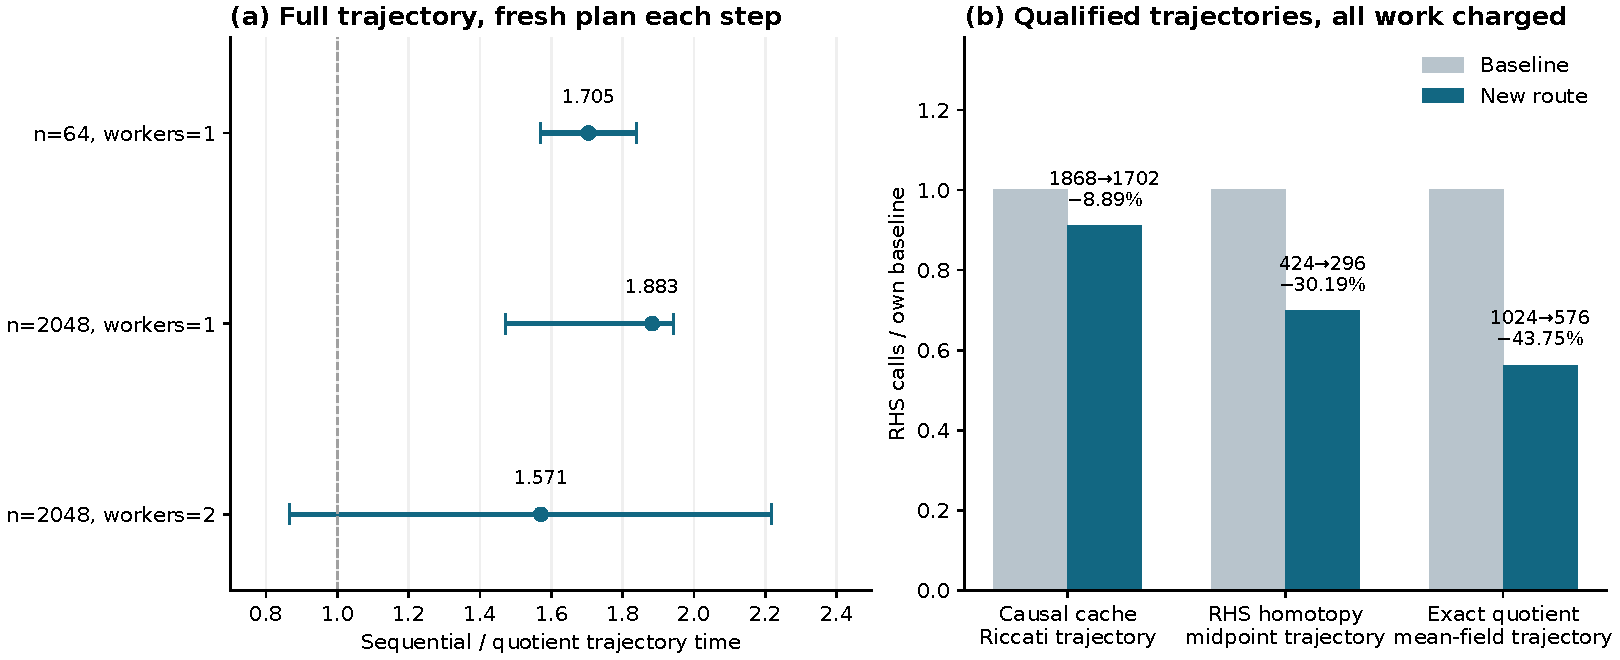
\includegraphics[width=.98\textwidth]{performance.pdf}
\caption{New measurements. Left: complete qualified structural trajectory
ratios including setup, allocation and the same full-space screen; horizontal
ranges are observed five-block extrema. Right: reductions in actual RHS work
for three different qualified trajectory cohorts. Each bar is normalized to
its own matched baseline and is not an across-problem solver ranking.}
\label{fig:performance}
\end{figure*}

Table~\ref{tab:structural-time} reports five ABBA/BAAB blocks per pair.
Native pools are created outside timers; model allocation, plan construction,
all steps, and full-space validation are inside. Retained observations and
JSON serialization are outside. At $n=2048$, one worker, fresh plans give a
median ratio 1.883 with block range $[1.472,1.943]$; reused plans give
1.891 with $[1.697,2.323]$. The two-worker fresh-plan range includes one.
These are shared-host observed ratios rather than confidence intervals or a
universal parallel speed claim.

\subsection{Residual tolerance derived from an accuracy specification}
The user's subsequent request for proof-derived constants is treated as a
separate changed-dependency extension; the original timing protocol remains
intact. The new \texttt{algebraic\_residual\_budget} method derives the sharp
finite-horizon residual amplification $C_N$ from the two scalar adjoints and
the two channel stability values proved above. A specified global algebraic
error budget $E_{\rm alg}$ then gives $\delta=E_{\rm alg}/C_N$ without a fitted
safety factor. The finite-horizon formula does not assume contraction.

An independent exact-rational audit checks twelve cells, including zero and
equal rates, forward-impulse/adjoint equality, sign-aligned norm extremizers,
and the exact 64-step budget identity. For $n=17$, $d=20$, $\kappa=19$,
$h=1/64$, its values are
\begin{align}
A_{17}&=23.233650367216686, &G_{17}&=0.9844964370054083,\\
C_{64}&=947.2963123944904,
&\delta(E_{\rm alg}=10^{-8})&=1.0556359049601808\times10^{-11}.
\end{align}
The native f64 implementation evaluates the same formulas, with the expected
last-bit differences. A new, untimed 64-step experiment under the derived
screen has maximum physical grid error $2.42381\times10^{-10}$ and
old/new difference $5.55112\times10^{-16}$; successful RHS counts remain
$1024\to576$. This is a precise algebraic residual-budget construction.
Its structural f64 constants and sampled residuals are not outward interval
certificates; evaluation and update roundoff require the separate terms
stated in the theorem.

The current structural API returns work on successful candidates. Its
\texttt{CoreResult} failures do not preserve a partial-work object.
These experiments therefore establish successful standalone trajectory cost.
Before coupling this API to a failed-attempt adaptive fallback, a charged
partial-work return contract is an explicit integration obligation.

\section{A direct-RHS homotopy corrector}

For a direct fixed-point map $G$, we implement
$G_\lambda(x)=(1-\lambda)a+\lambda G(x)$, with a fixed initial anchor $a$ and
an increasing station sequence ending at $\lambda=1$. The callback exposes
only map values. The native corrector requests no Jacobian, JVP, finite
difference derivative, AD, matrix factorization, or Newton solve. Its
depth-one Anderson trial is
\begin{align}
r&=G_\lambda(x)-x,\qquad \Delta r=r-r_{\rm old},\\
\gamma&=\frac{\langle r,\Delta r\rangle}{\|\Delta r\|^2},\\
e&=G_\lambda(x)-\gamma\left[G_\lambda(x)-G_\lambda(x_{\rm old})\right].
\end{align}
The Picard candidate $p=G_\lambda(x)$ is evaluated first. An admitted trial
replaces it only if its actual residual satisfies
$\|r_\lambda(e)\|\le\eta\|r_\lambda(p)\|$, with $0<\eta\le1$.
All trial evaluations are charged, including rejected trials. History is
reset at station changes. Anderson acceleration is established methodology;
the contribution here is the native direct-RHS contract, its safeguard, and
the measured connection to the solver's stage equations.

On a common invariant closed convex domain, if $G$ is $q$-Lipschitz and
$\lambda q<1$, then
\begin{equation}
\|r_\lambda(x_{j+1})\|\le\lambda q\|r_\lambda(x_j)\|,\qquad
\|x_j-x_\lambda^*\|\le\frac{\|r_\lambda(x_j)\|}{1-\lambda q}.
\end{equation}
Indeed, $r_\lambda(p)=G_\lambda(G_\lambda(x))-G_\lambda(x)$ is bounded by
$\lambda q\|r_\lambda(x)\|$, and the screen can only improve this bound.
The second inequality follows from the triangle inequality at the unique
fixed point. These are exact-arithmetic conditional statements; the code
reports operational binary64 residuals.

The nonlinear RK consumer solves the implicit-midpoint equation for
$y'=-ky-gy^3$, $k>0$, $g\ge0$:
\begin{equation}
F(K)=K+h\left[k(y+K/2)+g(y+K/2)^3\right]=0.
\end{equation}
For the zero-anchor station equation, $F_\lambda'\ge1+\lambda hk/2$;
hence $|K-K_\lambda^*|\le|F_\lambda(K)|/(1+\lambda hk/2)$, including
noncontractive Picard regimes. Monotone bisection supplies an independent
root oracle. The exact ODE solution
\begin{equation}
y(t)=\frac{y_0e^{-kt}}{\sqrt{1+(g/k)y_0^2(1-e^{-2kt})}}
\end{equation}
also scores every returned grid state.

The native contracts pass $11/11$. At stage residual tolerance $10^{-12}$,
scalar and 64-vector linear midpoint targets with $hk/2=0.99$ reduce vector
RHS calls from 2819 and 3029, respectively, to four. A nonlinear scalar target
uses 37 versus 12 calls; the nonlinear 64-vector target uses 495 versus 16
with the conditional proposal policy. These are same-stage-target work
comparisons, not physical-accuracy speedups at those coarse time steps.
All 24 full midpoint trajectories preserve the expected order two. At 64
steps the zero-seed Picard arm uses 424 calls and the warm-seed screened arm
296, a $30.19\%$ reduction, at maximum grid error approximately
$1.43644\times10^{-5}$.

Negative controls guide dispatch. The RK4 causal target needs 20 calls with
all-stage Picard, 36 with unconditional screened extrapolation, and only four
with exact forward evaluation. Intermediate homotopy stations increase the
easy nonlinear scalar solve from 12 to 28 calls. The noncontractive linear
Picard control reaches its 4096-update cap, whereas the screened affine
trial reaches the same root. No default policy or universal acceleration
claim follows from these finite cases.

\section{Physical budgets from analytic constants}

The user-directed extension adds a \texttt{ResidualDominance} policy with
$\eta=1$. It applies no fitted gain margin, observed-ratio threshold,
coefficient-magnitude cap, or rejection-count cap. The finite/domain checks
and the original residual evaluation remain. The older heuristic policies
are retained as controls. A separate sealed polynomial consumer derives its
step grid and residual target from the requested physical error budget;
no unproved global contraction factor is assigned to a generic RHS callback.

For $y'=-\Phi(y)$, $\Phi(y)=ky+gy^3$, $k>0$, $g\ge0$, and $y(0)=Y\ge0$,
the exact orbit stays in $[0,Y]$. The sharp derivative extrema on this interval
are
\begin{align}
M_1&=\Phi(Y),& L&=k+3gY^2,\\
M_2&=L\Phi(Y),&
M_3&=\Phi''(Y)\Phi(Y)^2+L^2\Phi(Y).
\end{align}
For an exact ODE increment, the midpoint stage residual is $A-B$, where
$A=h[\Phi((y_0+y_1)/2)-\Phi(y(h/2))]\ge0$ and
$B=\int_0^h\Phi(y(t))dt-h\Phi(y(h/2))\ge0$. Endpoint interpolation and
midpoint quadrature give $A\le h^3LM_2/8$ and $B\le h^3M_3/24$.
The exact polynomial identity
\begin{equation}
2\Phi'(Y)^2-\Phi''(Y)\Phi(Y)=2k^2+6kgY^2+12g^2Y^4\ge0
\end{equation}
implies $M_3\le3LM_2$. Taking the larger of the two positive-defect bounds
therefore gives
\begin{equation}
|F(K_{\rm exact\ ODE})|\le Ch^3,\qquad
C=\frac{L^2\Phi(Y)}8.
\end{equation}
This is a proved finite-step upper bound, not an optimal sharp truncation
constant. The factor $1/8$ is the interpolation remainder constant, not a fit.

Writing the ideal midpoint step as $\Psi_h(y)=2m-y$, where
$m+(h/2)\Phi(m)=y$, yields
\begin{equation}
\Psi_h'(y)=\frac{1-(h/2)\Phi'(m)}{1+(h/2)\Phi'(m)},
\qquad |\Psi_h'(y)|\le1.
\end{equation}
This global nonexpansivity transports algebraic errors without an assumed
Jacobian norm along the computed trajectory. With $D=1+hk/2$, the physical
error at step $n$ is bounded by $nCh^3/D+\sum_{j\le n}\alpha_j$.

For user budget $\epsilon$, the native plan selects the smallest dyadic $N$
such that represented $h=T/N$ is exact, $Nh=T$, and
\begin{equation}
E_{\rm trunc}=\frac{NCh^3}{D}<\epsilon,
\qquad q_B=\frac h2\left[k+3g(Y+\epsilon)^2\right]<1.
\end{equation}
The enlarged interval follows from the preceding physical-error induction.
The dyadic grid is an explicit representation constraint; minimality is
claimed only within that class. The remaining budget determines
\begin{equation}
\alpha_{\rm budget}=\frac{\epsilon-E_{\rm trunc}}N,
\qquad \tau_F=D\alpha_{\rm budget}.
\end{equation}
There is no guessed split of $\epsilon$ or station spacing. Direct
$\lambda=1$ is used: intermediate contraction cannot repair a noncontractive
final target, and here $q_B<1$ is already supplied by the proved step choice.

Each candidate receives an outward interval evaluation of the original
polynomial $F(K)$, divided by a lower bound for $D$, plus the represented
addition displacement in $\operatorname{fl}(y+K)$. A value-only monotone
bisection polish is available if this bound requires refinement. A residual
rounding floor produces refusal, preserving accepted points. The reported
grid bound additionally includes $M_1|\operatorname{fl}(nh)-nh|$ for time
labels. The native directed-arithmetic contract assumes correct binary64/FMA
operations, gradual underflow, and no invalidating reassociation.

\begin{table*}[t]
\caption{New physically accuracy-matched runs for $k=1,g=1/2,Y=T=1$.
All scientific budgets follow the formulas above. RHS and interval-polynomial
evaluations are reported separately. Zero and warm seeds use the same plan.}
\label{tab:cubic-physical-constants}
\begin{ruledtabular}
\begin{tabular}{rrllrrrr}
$\epsilon$ & $N$ & Policy & Seed & RHS & Interval & Max. grid error & Final bound\\
$10^{-3}$&64&Picard&zero&192&64&$5.063\times10^{-5}$&$4.143\times10^{-4}$\\
$10^{-3}$&64&Picard&warm&134&64&$8.011\times10^{-5}$&$4.710\times10^{-4}$\\
$10^{-3}$&64&Dominance&zero&192&64&$5.063\times10^{-5}$&$4.143\times10^{-4}$\\
$10^{-3}$&64&Dominance&warm&134&64&$8.011\times10^{-5}$&$4.710\times10^{-4}$\\
$10^{-4}$&128&Picard&zero&430&128&$3.664\times10^{-6}$&$8.014\times10^{-5}$\\
$10^{-4}$&128&Picard&warm&334&128&$3.834\times10^{-6}$&$7.931\times10^{-5}$\\
$10^{-4}$&128&Dominance&zero&430&128&$3.579\times10^{-6}$&$8.002\times10^{-5}$\\
$10^{-4}$&128&Dominance&warm&334&128&$3.831\times10^{-6}$&$7.930\times10^{-5}$\\
$10^{-5}$&512&Picard&zero&1580&512&$4.988\times10^{-7}$&$5.878\times10^{-6}$\\
$10^{-5}$&512&Picard&warm&1147&512&$7.086\times10^{-7}$&$6.095\times10^{-6}$\\
$10^{-5}$&512&Dominance&zero&1580&512&$4.991\times10^{-7}$&$5.877\times10^{-6}$\\
$10^{-5}$&512&Dominance&warm&1147&512&$7.086\times10^{-7}$&$6.095\times10^{-6}$\\
\end{tabular}
\end{ruledtabular}
\end{table*}

All twelve runs complete and every observed error lies below its outward
bound and requested cap. Decimal80 independently checks the constants,
remaining-budget inequalities, dyadic minimality, and exact-solution
observations. Seventeen distinct native contracts pass, including a focused
rounding-floor refusal. At $\epsilon=10^{-5}$, zero-seed Picard uses 2092
total polynomial evaluations and warm-seed dominance 1659, a $20.70\%$
reduction. The two policies have equal RHS counts for each seed on these
rapidly contractive grids; the savings here belong to accepted-stage reuse
under the derived physical budget. These counts do not assert equal cost per
ordinary versus interval evaluation, or a wall-clock speedup.

\begin{figure*}[t]\centering
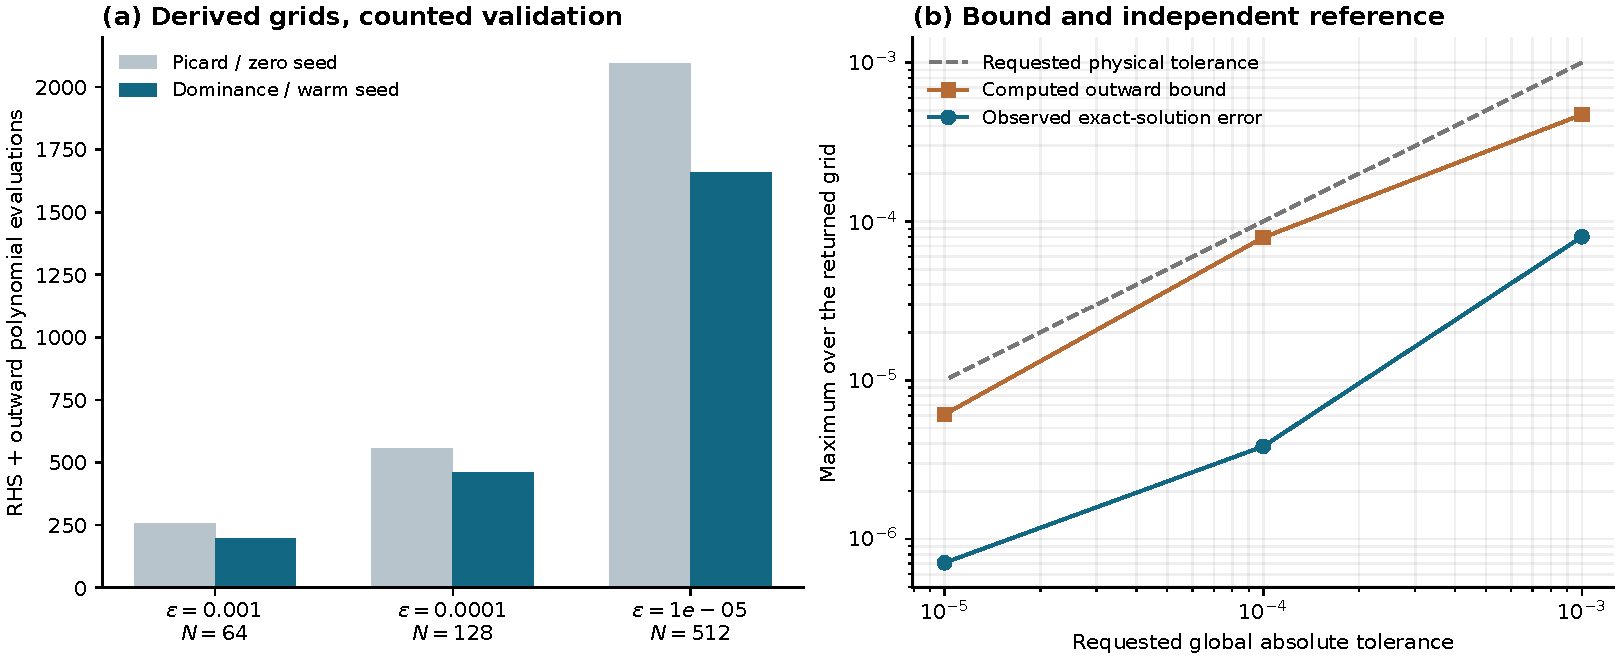
\includegraphics[width=.98\textwidth]{exact_constants.pdf}
\caption{Proof-derived physical-accuracy experiments for the sealed cubic
decay model. Every interval polynomial validation is charged. The four-arm
ablation in the text shows that the work decrease on these fast-contraction
grids comes from the warm seed; acceleration alone has equal evaluation
counts. Right: the computed outward error bound and the independent
closed-form error remain below the requested physical tolerance.}
\label{fig:exact-constants}
\end{figure*}

\section{Adapter policy and selective derivative use}
The adapter is analyzed independently of stage-root cost. The initial
control uses the existing \texttt{adaptive\_evidence(ProvidedOnly)} policy,
the PR90 dominance stop, and only a supplied JVP provider. Its equation is
$y'=-ry$ in sixteen identical components, $y_i(0)=1$, on $[0,1]$, at
$r=1,1000,10000$. Both arms retain $\mathrm{rtol}=10^{-7}$,
$\mathrm{atol}=10^{-10}$, $h_0=10^{-4}$ and eight common requested windows.
Every returned component is scored against $\exp(-rt)$ under $10^{-6}$.
All six initial solves passed. Callback atomics agree with the aggregate
RHS/JVP ledger. Jacobian builds and explicit-time derivative calls are zero.

At $r=1$, both routes use 79 RHS calls and zero JVPs. The initial evidence
policy is therefore truly RHS-only on the easy control. At $r=1000$ and
10000, however, the initially unmodified selector pays for losing JVP
pilots and stays explicit. Work rises from 2377 to 2958 and from 19261 to
20190. This is retained as a concrete adapter failure, rather than treated
as proof that derivative assistance is intrinsically inefficient.

The trace identifies a cold-start mechanism. At a late $r=1000$ checkpoint,
the persistent explicit session already proposes approximately
$3.662\times10^{-3}$, yet the same-checkpoint implicit pilot restarts from
$10^{-4}$. It exhausts the comparison work cap before completing the matched
interval. Existing post-pilot step reuse acts only after a pilot wins and
does not repair this entry reset.
The new opt-in checkpoint seed uses the positive finite step proposal stored
\emph{before} the explicit replay begins. It does not borrow the replay's
future final proposal. Only the initial pilot proposal changes; the native
error controller, endpoint, fatal precedence, and charged-work comparison
remain in force. Default settings are unchanged.

With the original entry ratio $0.8$, the repaired late pilots complete at
work 160, versus 192 for the explicit matched prefix, but $160/192=5/6>0.8$
still causes refusal. A separately declared post-diagnosis control therefore
tested strict local work improvement. The final implementation expresses this
as $C_{\rm pilot}<C_{\rm explicit}$ in checked integer arithmetic, rather than
using a nearly-one floating threshold. Equal costs retain the incumbent.
The break-even constant one follows from minimizing the declared work
objective; it is not fitted to this example.

The objective is the repository's existing accounting convention,
\begin{equation}
 C=N_f+N_{Jv}+N_{f_t}+nN_J+N_{\rm linear\ solve}.
\end{equation}
These unit weights define counted work, not a machine-independent time model.
The strict policy also derives a callback lower-bound ceiling of
$C_{\rm explicit}-1$. No incomplete or mismatched replay is admitted as a
winner. Tests distinguish ties and one-unit improvements above $2^{53}$ and
check overflow and safe ceiling behavior. The prior ratio path remains the
default; \texttt{strict\_entry\_work\_improvement} is independently opt-in.

\begin{table*}[t]\centering
\caption{Complete adaptive trajectories, including unsuccessful probes.
The strict arm combines checkpoint proposal reuse with exact local work
comparison. Every returned component passes the unchanged $10^{-6}$ cap.}
\begin{tabular}{r r r r r r r}\toprule
$r$ & RHS-only work & Initial selective & Seed only & Strict work & Strict RHS & Strict JVP\\\midrule
1 &79&79&79&79&79&0\\
1000 &2377&2958&2890&1691&1105&426\\
10000 &19261&20190&20094&1629&992&445\\
\bottomrule\end{tabular}\label{tab:adapter}\end{table*}

The two stiff cases reduce total charged work by $28.86\%$ and $91.54\%$
against the fully RHS-only baseline. Their maximum returned-state errors are
$1.06542\times10^{-9}$ and $1.31464\times10^{-9}$; these are larger than the
RHS-only errors but within the identical physical accuracy contract. The easy
case performs no JVP calls. All twelve arms complete, and the integer policy
reproduces all prior parity-control numerical outcomes, counters, states,
and times after excluding only descriptive policy metadata. This comparison
reports work, not elapsed-time acceleration.

The original six-arm failure, nine-arm seed ablation, and twelve-arm policy
control remain in the evidence. Selection of the strict policy followed the
trace diagnosis, so it is an exploratory repair experiment rather than a
held-out performance study. A local strict-work optimum does not prove an
optimal future route. Existing pressure, retry/backoff, return margins,
step-controller factors, and observation windows retain their original
heuristic or user-configuration status; they are not certified universal
constants by this change.


\begin{figure*}[t]\centering
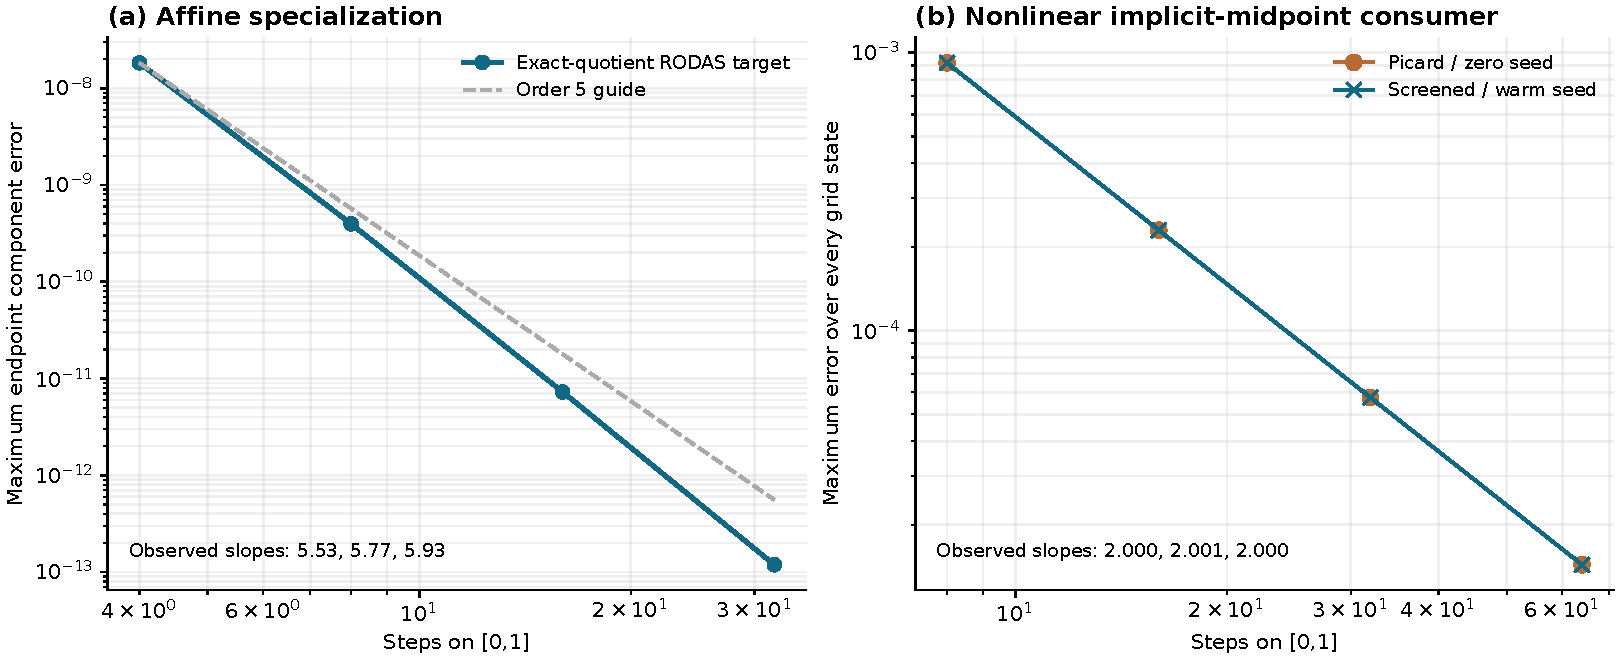
\includegraphics[width=.98\textwidth]{accuracy.pdf}
\caption{Independent exact-solution refinement checks. The structural affine
specialization preserves the original raw-stage target and exhibits the
listed restricted-family slopes. The nonlinear direct-RHS midpoint consumer
retains its second-order grid convergence, with baseline and improved curves
overlapping. A root accelerator changes the algebraic solution cost, not
the order of the chosen time discretization.}
\label{fig:accuracy}
\end{figure*}

\section{What the experiments decide}
The mathematical construction has useful exact structure. An acyclic
stage graph permits finite residual transport even when a global
Lipschitz contraction test fails. An exact declared quotient can eliminate
derivative callbacks and the full-state sequential stage sweep. An
actual-residual safeguard gives a clear conditional convergence proof for
a vector-only homotopy correction. These results are sufficient to justify
the implemented scoped paths and their experiments.

The retained failures identify where more theory or selection work is needed.
A general nonlinear client need not possess the mean-field quotient.
A near-closure requires a proved closure-defect term and an original-coordinate
error transport bound. Replacing the frozen derivative in a Rosenbrock target
by a convenient physical carrier generally changes the target; higher-order
conditions must then be derived for that method. The local sampled residual
is not a whole-domain or continuous-time certificate. General noncontractive
RHS maps require a root branch/domain argument or other residual-to-error
information; the cubic midpoint consumer has such a monotonicity argument,
whereas an arbitrary black-box map does not inherit it.

The successful optimization tasks have a different character. Reusing exact
inputs, unchanged solve prefixes, scalar plans, and checkpoint proposals
leaves the numerical targets or adaptive admission contracts intact.
Their remaining costs are measured. Cache metadata, parallel dispatch, and
extra residual trials can exceed savings on small/easy inputs, so negative
cells remain part of policy design.

No new global impossibility theorem is claimed. NG1--NG7 therefore do not
license promoting a failed fixture into a project-wide no-go result.
The closed V6/V8 physical campaigns and their global completion ledger are
unchanged; this unit's completion refers to the constructions, code, and
specified experiments above.

\section{Reproduction and evidence}
The research node contains the exact formulas, source snapshots, initial
and repaired failure logs, native execution receipts, full numerical
results, summary scripts, and this REVTeX source.
\texttt{REPRODUCE.md} gives precise commands and the retained evidence
archive layout. Rust 1.94.1 and the repository's locked offline dependencies
were used with \texttt{--profile measurement} (optimization level 3,
LTO disabled, sixteen codegen units). Cargo builds and timings were serialized.
An initial accidental debug-profile build consumed about 223 seconds.
A cancellation was requested, but the retained complete log records both
six-test suites finishing successfully. An earlier cancellation receipt
incorrectly described the final log as containing no tests. That conflicting
receipt is preserved and superseded by the provenance reconciliation; the
separate measurement-profile run remains the selected evidence and the debug
tests are not counted twice. The selected suites contain 59 distinct passing
native tests. A final locked offline compile of all targets in the two changed
crates also passes; it checks compatibility of the new public variants and
configuration fields and is not an additional timing experiment.

The source-only theory checks independently use exact fractions: 32
mean-field cells, 832 stage-component equalities, zero exact original-target
residual, a finite causal inverse with $\|L\|_\infty=13$, and twelve scalar
affine extrapolation controls. Wolfram verified the nilpotent inverse,
mean-field resolvent and scalar extrapolation identities. An initial
unevaluated zero-power expression was corrected and retained as a tool
expression failure. SciSpace and Exa were used to find primary literature;
source claims were checked against the original papers.

\begin{thebibliography}{9}
\bibitem{vdH1991}
P. J. van der Houwen and B. P. Sommeijer,
Iterated Runge--Kutta methods on parallel computers,
SIAM J. Sci. Stat. Comput. \textbf{12}, 1000--1028 (1991).
\url{https://ir.cwi.nl/pub/1589/1589D.pdf}.
\bibitem{pollock2021}
S. Pollock and L. G. Rebholz,
Anderson acceleration for contractive and noncontractive operators,
IMA J. Numer. Anal. \textbf{41}, 2841--2872 (2021),
\href{https://doi.org/10.1093/imanum/draa095}{doi:10.1093/imanum/draa095}.
\bibitem{tranquilli2014}
P. Tranquilli and A. Sandu,
Rosenbrock--Krylov methods for large systems of differential equations,
SIAM J. Sci. Comput. \textbf{36}, A1313--A1338 (2014),
\href{https://doi.org/10.1137/130923336}{doi:10.1137/130923336}.
\bibitem{walker2011}
H. F. Walker and P. Ni,
Anderson acceleration for fixed-point iterations,
SIAM J. Numer. Anal. \textbf{49}, 1715--1735 (2011).
\end{thebibliography}
\end{document}
